\section{Risikomanagement}

\subsection{Risiken}
\begin{figure}[H]
	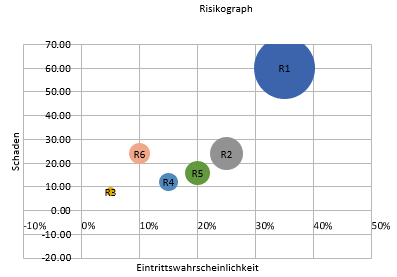
\includegraphics[width=\textwidth,height=\textheight,keepaspectratio]{images/Risikoanalyse_vorher.png}
	\caption{Ursprüngliche Risikoanalyse}
\end{figure}

\noindent Die detailierte Risikoanalyse kann dem Dokument ''TechnischeRisiken.pdf'' entnommen werden.

\subsection{Umgang mit Risiken}
Risiken lassen sich in einem grösseren Projekt leider nicht vermeiden. Allfällige Risiken werden jeweils zu Beginn eines Sprints im Team angesprochen und sofern sinnvoll wurden dementsprechend Massnahmen getroffen.
\\
\\
Für die wahrscheinlichen Risiken wurden Massnahmen definiert, um den auftretetenden Schaden unter Kontrolle zu bringen. Sollten während des Projektes neue Risiken hervortreten, werden diese in die Risikoanalyse aufgenommen und bewertet.

\newpage